% ==========================================
% CHƯƠNG 5: THỰC NGHIỆM VÀ KẾT QUẢ
% ==========================================
\chapter{THỰC NGHIỆM VÀ KẾT QUẢ}

\section{Xây dựng bộ dữ liệu và kỹ thuật tăng cường dữ liệu}

Để xây dựng mô hình có khả năng tổng quát hóa tốt trong nhiều điều kiện thực tế,
nhóm nghiên cứu sử dụng kết hợp hai nguồn dữ liệu: bộ dữ liệu chuẩn QIPEDC (Bộ
dữ liệu ngôn ngữ ký hiệu dành cho giáo dục học sinh khiếm thính cấp tiểu học của
Bộ GD\&ĐT) và bộ dữ liệu tự thu thập thông qua công cụ quay video được nhóm xây
dựng. Dữ liệu tự thu thập được thiết kế theo cùng cấu trúc và định dạng của
QIPEDC nhằm đảm bảo tính nhất quán khi kết hợp hai nguồn. Bộ dữ liệu cuối cùng
bao gồm 108 lớp ký hiệu với tổng cộng 10.800 video gốc trước khi tăng cường.

Quá trình thu thập được thiết kế có chủ đích: mỗi từ/cụm từ được quay với đầy đủ
7 trạng thái cảm xúc (angry, disgust, fear, happy, sad, surprise, neutral) bởi
nhiều người thực hiện khác nhau, với góc quay và điều kiện ánh sáng đa dạng.
Đây là bước nền tảng quan trọng giúp mô hình học được sự phong phú của biểu đạt
cảm xúc trong VSL.

Toàn bộ dữ liệu được chia theo tỉ lệ 70\% Train -- 15\% Val -- 15\% Test.
Tập Train được dùng để huấn luyện mô hình, tập Val để theo dõi quá trình hội tụ
và chọn checkpoint tốt nhất, tập Test hoàn toàn độc lập chỉ được dùng một lần
duy nhất để báo cáo kết quả cuối cùng.

Chiến lược tăng cường dữ liệu sinh ra 9 biến thể từ mỗi video gốc, chỉ áp dụng
trên tập Train; tập Val và Test giữ nguyên dữ liệu gốc không qua tăng cường nhằm
đảm bảo đánh giá khách quan hiệu năng thực sự của mô hình trong điều kiện triển
khai thực tế. Chín biến thể bao gồm:
\textit{(1)} file gốc,
\textit{(2)} mirror hoán đổi tay trái $\leftrightarrow$ tay phải,
\textit{(3)} mirror kết hợp nhiễu Gaussian,
\textit{(4--5)} nhiễu Gaussian hai mức (0.003 và 0.006) tác động lên tọa độ xyz,
\textit{(6--7)} co giãn tỷ lệ tay ($\times$0.95 và $\times$1.05) để mô phỏng
khoảng cách người dùng đến camera,
\textit{(8--9)} time warp cắt 5\% và 10\% đầu/cuối để học tốc độ thực hiện
ký hiệu khác nhau.
Mirror augmentation là kỹ thuật đặc biệt quan trọng giúp mô hình tổng quát hóa
với cả người thuận tay trái lẫn tay phải mà không cần thu thập thêm dữ liệu.
Nhờ chiến lược này, số lượng mẫu huấn luyện tăng gấp 9 lần so với dữ liệu gốc.

Hình~\ref{fig:data_dist} minh họa phân phối số lượng mẫu theo từng lớp sau khi
tăng cường. Có thể thấy các lớp tương đối cân bằng nhau, hạn chế hiện tượng
lệch lớp trong quá trình huấn luyện.

\begin{figure}[ht]
    \centering
    
\includegraphics[width=\textwidth]{images/5_data_distribution.png}
    \caption{Biểu đồ phân phối mẫu theo từng lớp ký hiệu}
    \label{fig:data_dist}
\end{figure}

% ─────────────────────────────────────────────────────────────────
\section{Kết quả huấn luyện}
% ─────────────────────────────────────────────────────────────────

Quá trình huấn luyện được thực hiện trên framework PyTorch với optimizer AdamW,
learning rate khởi đầu $5 \times 10^{-4}$, warmup tuyến tính 8 epoch và cosine
decay về $10^{-6}$. Gradient clipping 1.0 và label smoothing 0.1 được áp dụng
để ổn định quá trình hội tụ. Early stopping với patience 20 epoch được sử dụng
để tránh lãng phí tài nguyên tính toán khi mô hình đã hội tụ.

Hình~\ref{fig:training_curves} thể hiện đường cong loss và accuracy trên tập
Train và Val. Mô hình hội tụ ổn định sau 60 epoch, đạt độ chính xác validation
tốt nhất 99.4\% tại epoch 41. Khoảng cách nhỏ giữa đường train và val cho thấy
mô hình không bị overfitting, chiến lược dropout (0.2) và label smoothing đã
phát huy hiệu quả trong việc kiểm soát độ phức tạp của mô hình.

\begin{figure}[ht]
    \centering
    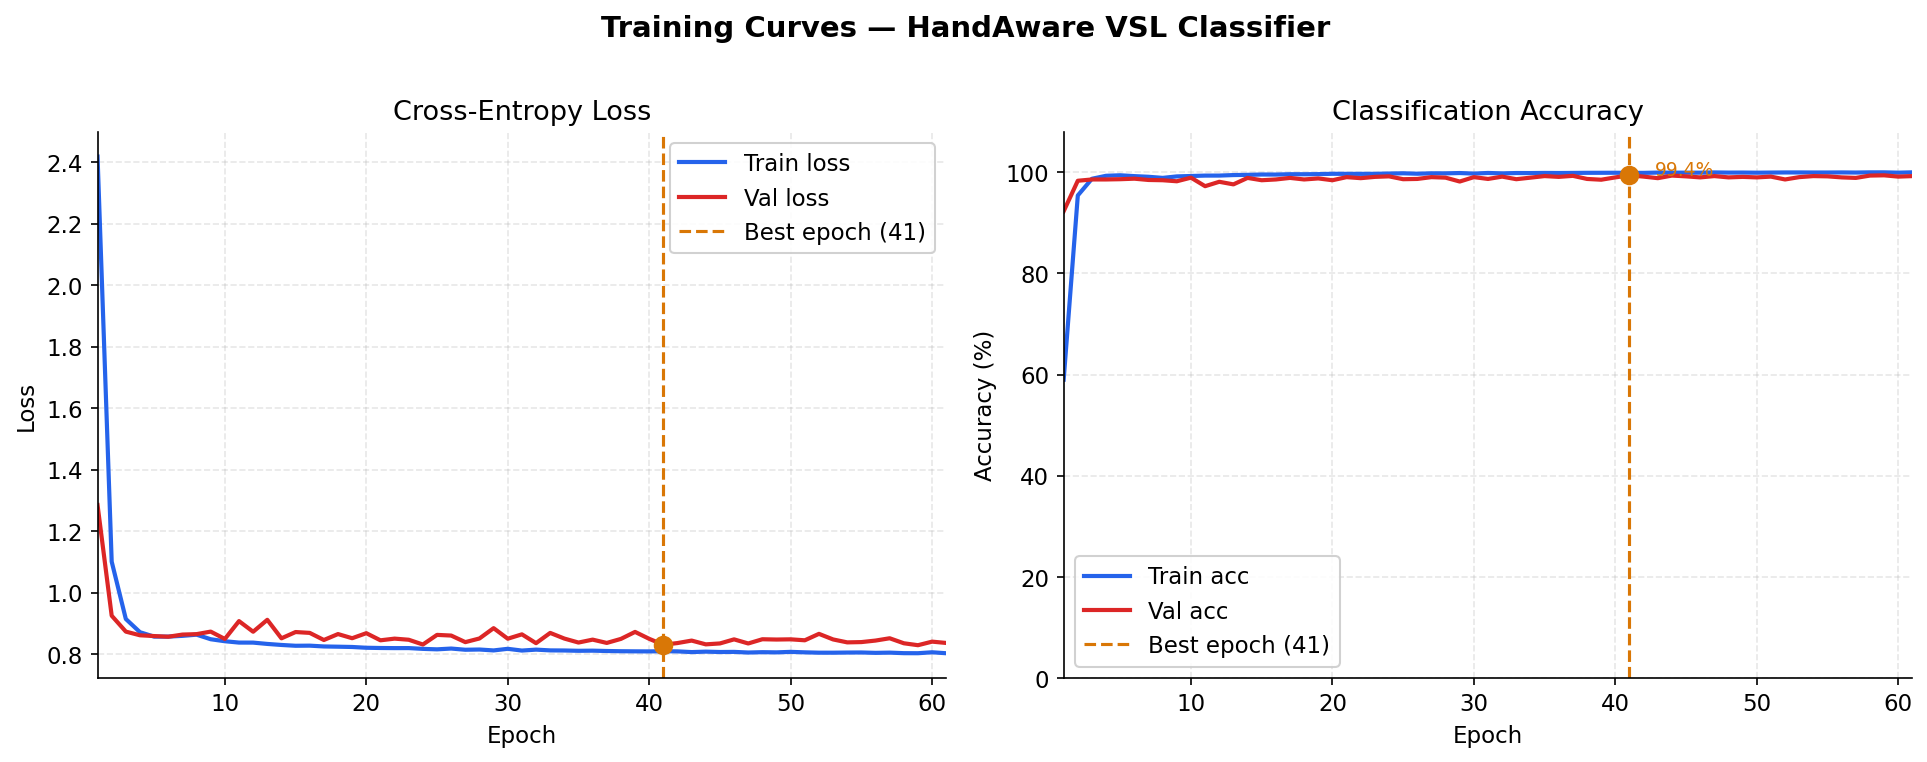
\includegraphics[width=\textwidth]{images/1_training_curves.png}
    \caption{Biểu đồ đường cong huấn luyện}
    \label{fig:training_curves}
\end{figure}

% ─────────────────────────────────────────────────────────────────
\section{Đánh giá trên tập kiểm thử}
% ─────────────────────────────────────────────────────────────────

Mô hình tốt nhất (checkpoint tại epoch 41 với val accuracy 99.4\%) được nạp lại
để đánh giá trên tập Test hoàn toàn độc lập. Kết quả tổng hợp được trình bày
trong Bảng~\ref{tab:results}.

\begin{table}[ht]
\centering
\caption{Kết quả đánh giá mô hình HandAwareVSLClassifier trên tập Test}
\label{tab:results}
\begin{tabularx}{\textwidth}{l >{\centering\arraybackslash}X
                               >{\centering\arraybackslash}X
                               >{\centering\arraybackslash}X
                               >{\centering\arraybackslash}X}
\hline
\textbf{Mô hình} & \textbf{Accuracy} & \textbf{Precision}
    & \textbf{Recall} & \textbf{F1} \\
\hline
HandAwareVSLClassifier (208 dim)
    & 99.39\% & 99.12\% & 99.06\% & 99.06\% \\
\hline
\end{tabularx}
\end{table}

Hình~\ref{fig:confusion} trình bày ma trận nhầm lẫn được chuẩn hóa theo hàng
trên toàn bộ tập Test. Đường chéo chính có giá trị cao cho thấy phần lớn các
lớp được phân loại chính xác. Một số nhầm lẫn nhỏ tập trung ở các cặp ký hiệu
có cấu hình bàn tay tương đồng, phản ánh đúng thách thức ngôn ngữ học vốn có
của VSL -- nơi sự khác biệt giữa các ký hiệu đôi khi chỉ nằm ở góc độ bàn tay
hoặc chuyển động nhỏ của ngón tay.

\begin{figure}[ht]
    \centering
    \includegraphics[width=\textwidth]{images/3_confusion_matrix.png}
    \caption{Biểu đồ ma trận nhầm lẫn trên tập Test}
    \label{fig:confusion}
\end{figure}

Để đánh giá chi tiết hơn theo từng lớp, Hình~\ref{fig:per_class} thể hiện
Precision, Recall và F1-score của từng ký hiệu riêng lẻ. Macro F1 đạt 99.06\%,
cho thấy mô hình hoạt động nhất quán trên tất cả các lớp chứ không chỉ tốt ở
các lớp có nhiều mẫu. Đường kẻ đứt nét trong biểu đồ đánh dấu ngưỡng F1 = 80\%
-- hầu hết các lớp đều vượt ngưỡng này, chỉ một số ít lớp có F1 thấp hơn do
đặc thù về độ phức tạp của ký hiệu.

\begin{figure}[ht]
    \centering
    
\includegraphics[width=\textwidth]{images/4_per_class_metrics.png}
    \caption{Biểu đồ chỉ số từng lớp ký hiệu trên tập Test}
    \label{fig:per_class}
\end{figure}

% ─────────────────────────────────────────────────────────────────
\section{Phân tích định tính -- Temporal Attention}
% ─────────────────────────────────────────────────────────────────

Ngoài các chỉ số định lượng, nhóm nghiên cứu thực hiện phân tích định tính thông
qua trực quan hóa trọng số Temporal Attention nhằm hiểu rõ hơn cơ chế ra quyết
định của mô hình.

Hình~\ref{fig:attention} trực quan hóa trọng số Temporal Attention trên 16 mẫu
từ tập Test. Mỗi hàng là một mẫu, mỗi cột là một frame trong chuỗi 64 frame;
màu càng đậm biểu thị frame được mô hình chú ý nhiều hơn.

\begin{figure}[ht]
    \centering
    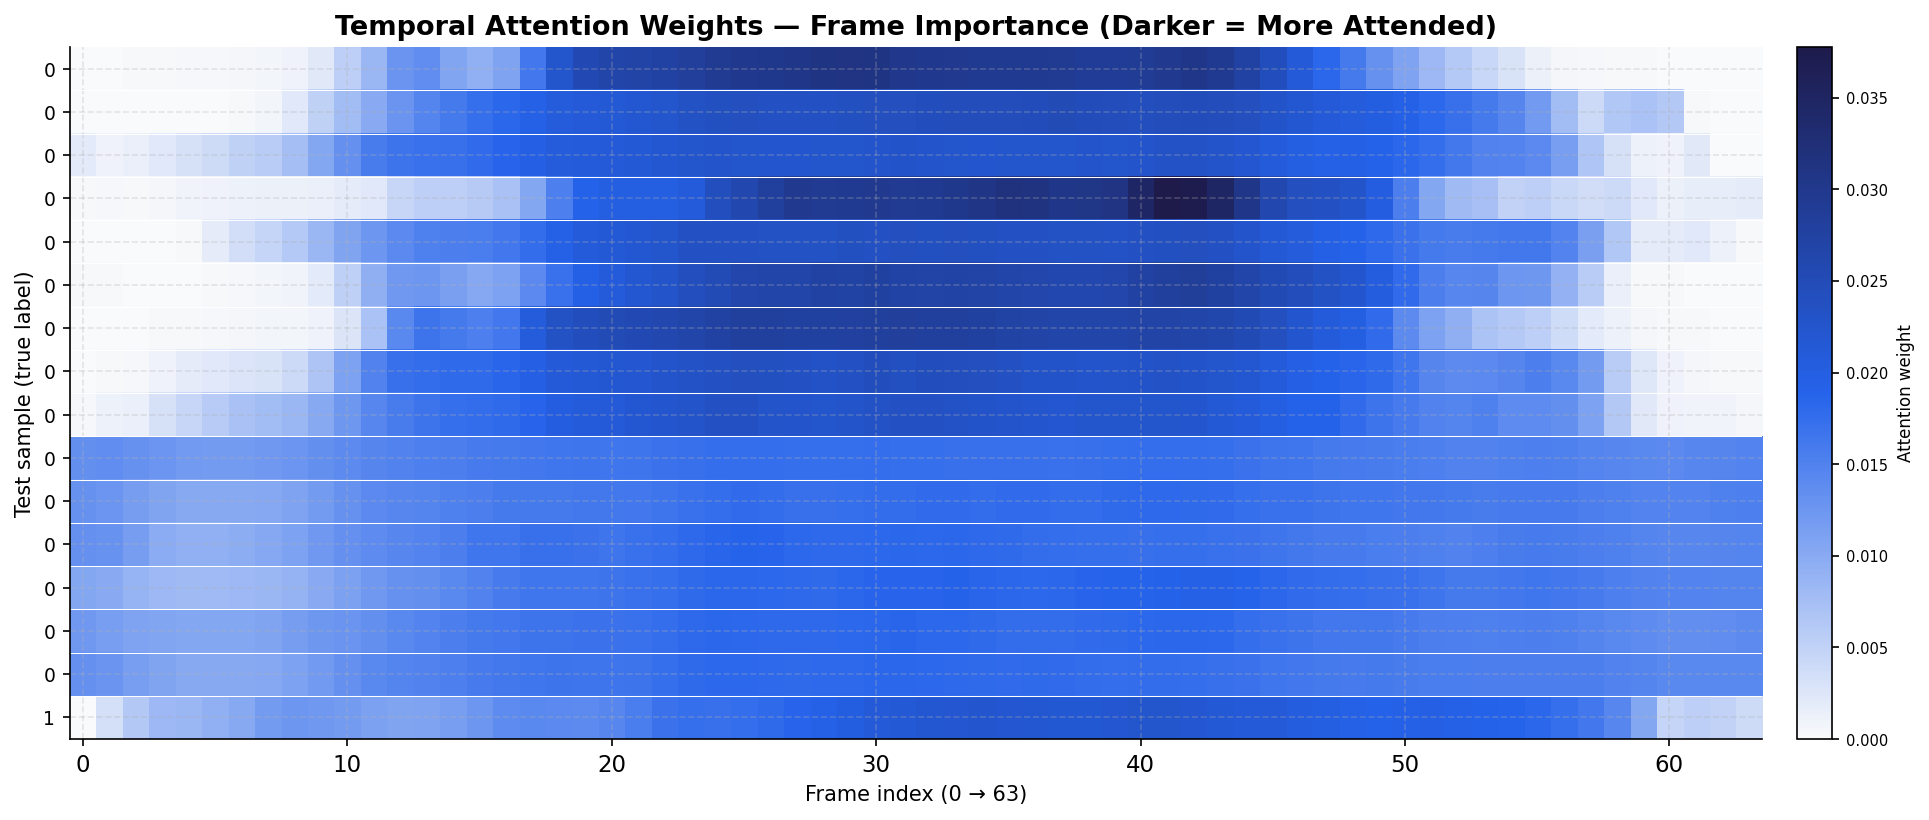
\includegraphics[width=\textwidth]{images/7_attention_weights.png}
    \caption{Biểu đồ trọng số Temporal Attention theo từng frame}
    \label{fig:attention}
\end{figure}

Có thể quan sát thấy mô hình tập trung chủ yếu vào các frame ở giữa chuỗi --
nơi cử chỉ ký hiệu được thực hiện đầy đủ và rõ ràng nhất -- trong khi các frame
đầu và cuối (thường là tư thế chuẩn bị và kết thúc) nhận trọng số thấp hơn.
Hành vi này hoàn toàn phù hợp với đặc điểm tự nhiên của ngôn ngữ ký hiệu: người
thực hiện thường có một khoảng chuyển tiếp trước và sau mỗi ký hiệu mà không
mang thông tin ngữ nghĩa. Điều này cho thấy cơ chế Temporal Attention Pooling
đã học được đặc điểm quan trọng này một cách tự động, không cần nhãn giám sát
về vị trí bắt đầu và kết thúc ký hiệu.

% ─────────────────────────────────────────────────────────────────
\section{Đánh giá vai trò của Emotion Encoding}
% ─────────────────────────────────────────────────────────────────

Một đóng góp quan trọng của đề tài là việc tích hợp 7 chiều Emotion vào feature
vector (từ 201 lên 208 chiều), bổ sung thông tin biểu cảm khuôn mặt vào quá
trình nhận dạng. Trong VSL, biểu cảm khuôn mặt là thành phần ngữ pháp bắt buộc
có khả năng thay đổi hoàn toàn ý nghĩa của một cử chỉ -- điều mà các hệ thống
chỉ dựa trên nhận diện tay thuần túy hoàn toàn bỏ sót.

Ví dụ điển hình là cặp ký hiệu ``Cảm ơn'' và ``Ghét'': hai ký hiệu này có cấu
hình tay gần như giống hệt nhau, chỉ khác nhau ở biểu cảm khuôn mặt
(HAPPY/NEUTRAL so với ANGRY). Nhờ tích hợp Emotion Encoding, mô hình có thể
phân biệt được các cặp ký hiệu đồng hình này một cách chính xác, góp phần vào
kết quả Macro F1 đạt 99.06\% trên tập Test.

Kết quả này minh chứng cho giả thuyết ban đầu rằng biểu cảm khuôn mặt không
thể bỏ qua trong bất kỳ hệ thống nhận dạng ngôn ngữ ký hiệu nghiêm túc nào.